\documentclass[1p]{elsarticle_modified}
%\bibliographystyle{elsarticle-num}

%\usepackage[colorlinks]{hyperref}
%\usepackage{abbrmath_seonhwa} %\Abb, \Ascr, \Acal ,\Abf, \Afrak
\usepackage{amsfonts}
\usepackage{amssymb}
\usepackage{amsmath}
\usepackage{amsthm}
\usepackage{scalefnt}
\usepackage{amsbsy}
\usepackage{kotex}
\usepackage{caption}
\usepackage{subfig}
\usepackage{color}
\usepackage{graphicx}
\usepackage{xcolor} %% white, black, red, green, blue, cyan, magenta, yellow
\usepackage{float}
\usepackage{setspace}
\usepackage{hyperref}

\usepackage{tikz}
\usetikzlibrary{arrows}

\usepackage{multirow}
\usepackage{array} % fixed length table
\usepackage{hhline}

%%%%%%%%%%%%%%%%%%%%%
\makeatletter
\renewcommand*\env@matrix[1][\arraystretch]{%
	\edef\arraystretch{#1}%
	\hskip -\arraycolsep
	\let\@ifnextchar\new@ifnextchar
	\array{*\c@MaxMatrixCols c}}
\makeatother %https://tex.stackexchange.com/questions/14071/how-can-i-increase-the-line-spacing-in-a-matrix
%%%%%%%%%%%%%%%

\usepackage[normalem]{ulem}

\newcommand{\msout}[1]{\ifmmode\text{\sout{\ensuremath{#1}}}\else\sout{#1}\fi}
%SOURCE: \msout is \stkout macro in https://tex.stackexchange.com/questions/20609/strikeout-in-math-mode

\newcommand{\cancel}[1]{
	\ifmmode
	{\color{red}\msout{#1}}
	\else
	{\color{red}\sout{#1}}
	\fi
}

\newcommand{\add}[1]{
	{\color{blue}\uwave{#1}}
}

\newcommand{\replace}[2]{
	\ifmmode
	{\color{red}\msout{#1}}{\color{blue}\uwave{#2}}
	\else
	{\color{red}\sout{#1}}{\color{blue}\uwave{#2}}
	\fi
}

\newcommand{\Sol}{\mathcal{S}} %segment
\newcommand{\D}{D} %diagram
\newcommand{\A}{\mathcal{A}} %arc


%%%%%%%%%%%%%%%%%%%%%%%%%%%%%5 test

\def\sl{\operatorname{\textup{SL}}(2,\Cbb)}
\def\psl{\operatorname{\textup{PSL}}(2,\Cbb)}
\def\quan{\mkern 1mu \triangleright \mkern 1mu}

\theoremstyle{definition}
\newtheorem{thm}{Theorem}[section]
\newtheorem{prop}[thm]{Proposition}
\newtheorem{lem}[thm]{Lemma}
\newtheorem{ques}[thm]{Question}
\newtheorem{cor}[thm]{Corollary}
\newtheorem{defn}[thm]{Definition}
\newtheorem{exam}[thm]{Example}
\newtheorem{rmk}[thm]{Remark}
\newtheorem{alg}[thm]{Algorithm}

\newcommand{\I}{\sqrt{-1}}
\begin{document}

%\begin{frontmatter}
%
%\title{Boundary parabolic representations of knots up to 8 crossings}
%
%%% Group authors per affiliation:
%\author{Yunhi Cho} 
%\address{Department of Mathematics, University of Seoul, Seoul, Korea}
%\ead{yhcho@uos.ac.kr}
%
%
%\author{Seonhwa Kim} %\fnref{s_kim}}
%\address{Center for Geometry and Physics, Institute for Basic Science, Pohang, 37673, Korea}
%\ead{ryeona17@ibs.re.kr}
%
%\author{Hyuk Kim}
%\address{Department of Mathematical Sciences, Seoul National University, Seoul 08826, Korea}
%\ead{hyukkim@snu.ac.kr}
%
%\author{Seokbeom Yoon}
%\address{Department of Mathematical Sciences, Seoul National University, Seoul, 08826,  Korea}
%\ead{sbyoon15@snu.ac.kr}
%
%\begin{abstract}
%We find all boundary parabolic representation of knots up to 8 crossings.
%
%\end{abstract}
%\begin{keyword}
%    \MSC[2010] 57M25 
%\end{keyword}
%
%\end{frontmatter}

%\linenumbers
%\tableofcontents
%
\newcommand\colored[1]{\textcolor{white}{\rule[-0.35ex]{0.8em}{1.4ex}}\kern-0.8em\color{red} #1}%
%\newcommand\colored[1]{\textcolor{white}{ #1}\kern-2.17ex	\textcolor{white}{ #1}\kern-1.81ex	\textcolor{white}{ #1}\kern-2.15ex\color{red}#1	}

{\Large $\underline{12a_{0713}~(K12a_{0713})}$}

\setlength{\tabcolsep}{10pt}
\renewcommand{\arraystretch}{1.6}
\vspace{1cm}\begin{tabular}{m{100pt}>{\centering\arraybackslash}m{274pt}}
\multirow{5}{120pt}{
	\centering
	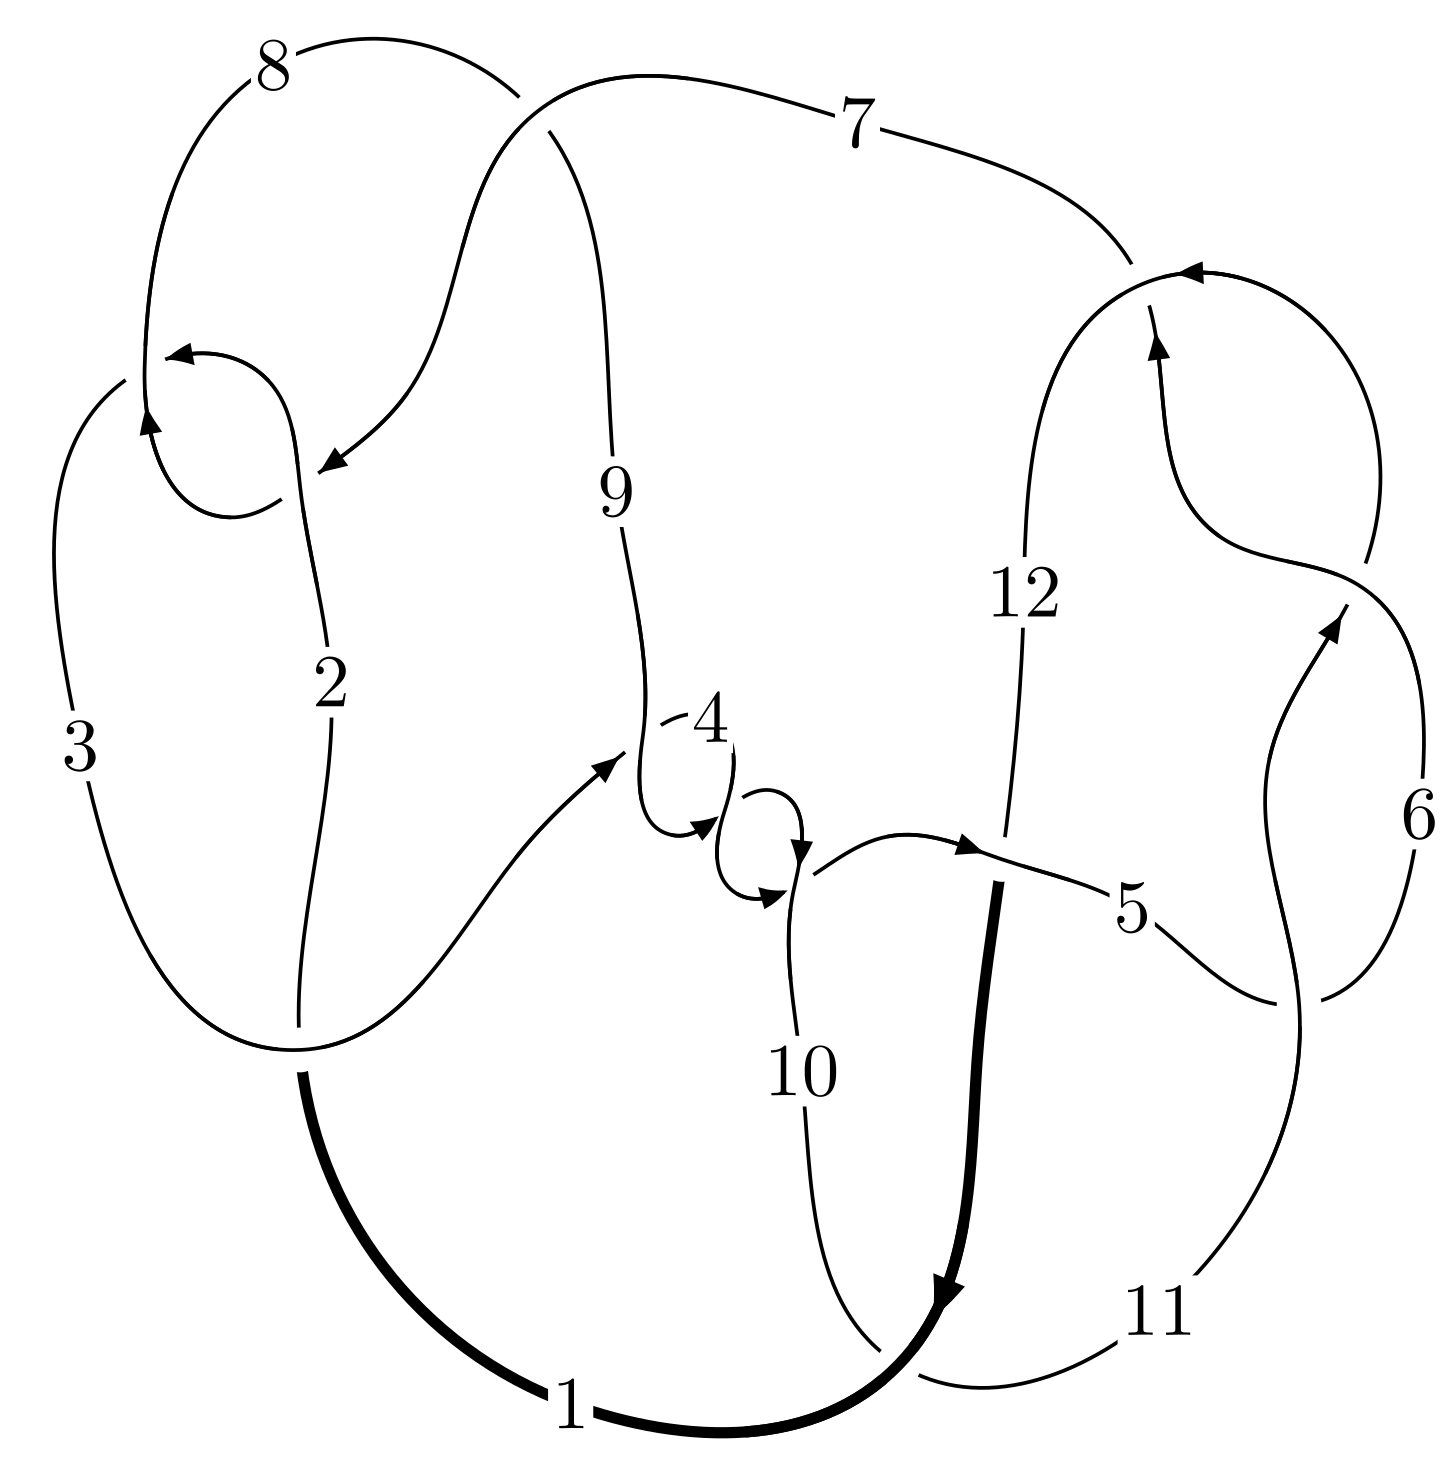
\includegraphics[width=112pt]{../../../GIT/diagram.site/Diagrams/png/1514_12a_0713.png}\\
\ \ \ A knot diagram\footnotemark}&
\allowdisplaybreaks
\textbf{Linearized knot diagam} \\
\cline{2-2}
 &
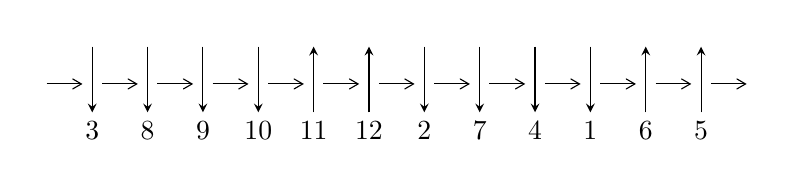
\begin{tikzpicture}[x=20pt, y=17pt]
	% nodes
	\node (C0) at (0, 0) {};
	\node (C1) at (1, 0) {};
	\node (C1U) at (1, +1) {};
	\node (C1D) at (1, -1) {3};

	\node (C2) at (2, 0) {};
	\node (C2U) at (2, +1) {};
	\node (C2D) at (2, -1) {8};

	\node (C3) at (3, 0) {};
	\node (C3U) at (3, +1) {};
	\node (C3D) at (3, -1) {9};

	\node (C4) at (4, 0) {};
	\node (C4U) at (4, +1) {};
	\node (C4D) at (4, -1) {10};

	\node (C5) at (5, 0) {};
	\node (C5U) at (5, +1) {};
	\node (C5D) at (5, -1) {11};

	\node (C6) at (6, 0) {};
	\node (C6U) at (6, +1) {};
	\node (C6D) at (6, -1) {12};

	\node (C7) at (7, 0) {};
	\node (C7U) at (7, +1) {};
	\node (C7D) at (7, -1) {2};

	\node (C8) at (8, 0) {};
	\node (C8U) at (8, +1) {};
	\node (C8D) at (8, -1) {7};

	\node (C9) at (9, 0) {};
	\node (C9U) at (9, +1) {};
	\node (C9D) at (9, -1) {4};

	\node (C10) at (10, 0) {};
	\node (C10U) at (10, +1) {};
	\node (C10D) at (10, -1) {1};

	\node (C11) at (11, 0) {};
	\node (C11U) at (11, +1) {};
	\node (C11D) at (11, -1) {6};

	\node (C12) at (12, 0) {};
	\node (C12U) at (12, +1) {};
	\node (C12D) at (12, -1) {5};
	\node (C13) at (13, 0) {};

	% arrows
	\draw[->,>={angle 60}]
	(C0) edge (C1) (C1) edge (C2) (C2) edge (C3) (C3) edge (C4) (C4) edge (C5) (C5) edge (C6) (C6) edge (C7) (C7) edge (C8) (C8) edge (C9) (C9) edge (C10) (C10) edge (C11) (C11) edge (C12) (C12) edge (C13) ;	\draw[->,>=stealth]
	(C1U) edge (C1D) (C2U) edge (C2D) (C3U) edge (C3D) (C4U) edge (C4D) (C5D) edge (C5U) (C6D) edge (C6U) (C7U) edge (C7D) (C8U) edge (C8D) (C9U) edge (C9D) (C10U) edge (C10D) (C11D) edge (C11U) (C12D) edge (C12U) ;
	\end{tikzpicture} \\
\hhline{~~} \\& 
\textbf{Solving Sequence} \\ \cline{2-2} 
 &
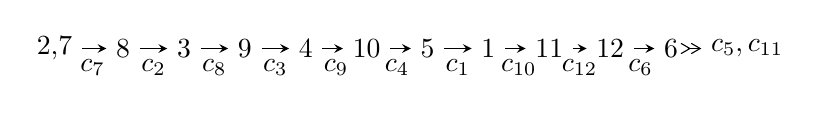
\begin{tikzpicture}[x=22pt, y=7pt]
	% node
	\node (A0) at (-1/8, 0) {2,7};
	\node (A1) at (1, 0) {8};
	\node (A2) at (2, 0) {3};
	\node (A3) at (3, 0) {9};
	\node (A4) at (4, 0) {4};
	\node (A5) at (5, 0) {10};
	\node (A6) at (6, 0) {5};
	\node (A7) at (7, 0) {1};
	\node (A8) at (8, 0) {11};
	\node (A9) at (9, 0) {12};
	\node (A10) at (10, 0) {6};
	\node (C1) at (1/2, -1) {$c_{7}$};
	\node (C2) at (3/2, -1) {$c_{2}$};
	\node (C3) at (5/2, -1) {$c_{8}$};
	\node (C4) at (7/2, -1) {$c_{3}$};
	\node (C5) at (9/2, -1) {$c_{9}$};
	\node (C6) at (11/2, -1) {$c_{4}$};
	\node (C7) at (13/2, -1) {$c_{1}$};
	\node (C8) at (15/2, -1) {$c_{10}$};
	\node (C9) at (17/2, -1) {$c_{12}$};
	\node (C10) at (19/2, -1) {$c_{6}$};
	\node (A11) at (45/4, 0) {$c_{5},c_{11}$};

	% edge
	\draw[->,>=stealth]	
	(A0) edge (A1) (A1) edge (A2) (A2) edge (A3) (A3) edge (A4) (A4) edge (A5) (A5) edge (A6) (A6) edge (A7) (A7) edge (A8) (A8) edge (A9) (A9) edge (A10) ;
	\draw[->>,>={angle 60}]	
	(A10) edge (A11);
\end{tikzpicture} \\ 

\end{tabular} \\

\footnotetext{
The image of knot diagram is generated by the software ``\textbf{Draw programme}" developed by Andrew Bartholomew(\url{http://www.layer8.co.uk/maths/draw/index.htm\#Running-draw}), where we modified some parts for our purpose(\url{https://github.com/CATsTAILs/LinksPainter}).
}\phantom \\ \newline 
\centering \textbf{Ideals for irreducible components\footnotemark of $X_{\text{par}}$} 
 
\begin{align*}
I^u_{1}&=\langle 
u^{69}+u^{68}+\cdots+u+1\rangle \\
\\
\end{align*}
\raggedright * 1 irreducible components of $\dim_{\mathbb{C}}=0$, with total 69 representations.\\
\footnotetext{All coefficients of polynomials are rational numbers. But the coefficients are sometimes approximated in decimal forms when there is not enough margin.}
\newpage
\renewcommand{\arraystretch}{1}
\centering \section*{I. $I^u_{1}= \langle u^{69}+u^{68}+\cdots+u+1 \rangle$}
\flushleft \textbf{(i) Arc colorings}\\
\begin{tabular}{m{7pt} m{180pt} m{7pt} m{180pt} }
\flushright $a_{2}=$&$\begin{pmatrix}0\\u\end{pmatrix}$ \\
\flushright $a_{7}=$&$\begin{pmatrix}1\\0\end{pmatrix}$ \\
\flushright $a_{8}=$&$\begin{pmatrix}1\\u^2\end{pmatrix}$ \\
\flushright $a_{3}=$&$\begin{pmatrix}- u\\- u^3+u\end{pmatrix}$ \\
\flushright $a_{9}=$&$\begin{pmatrix}- u^2+1\\u^2\end{pmatrix}$ \\
\flushright $a_{4}=$&$\begin{pmatrix}u^7-2 u^5+2 u^3-2 u\\- u^7+u^5-2 u^3+u\end{pmatrix}$ \\
\flushright $a_{10}=$&$\begin{pmatrix}u^{12}-3 u^{10}+5 u^8-6 u^6+4 u^4-3 u^2+1\\- u^{12}+2 u^{10}-4 u^8+4 u^6-3 u^4+2 u^2\end{pmatrix}$ \\
\flushright $a_{5}=$&$\begin{pmatrix}- u^{17}+4 u^{15}-9 u^{13}+14 u^{11}-15 u^9+14 u^7-10 u^5+6 u^3-3 u\\u^{17}-3 u^{15}+7 u^{13}-10 u^{11}+11 u^9-10 u^7+6 u^5-4 u^3+u\end{pmatrix}$ \\
\flushright $a_{1}=$&$\begin{pmatrix}u^3\\u^5- u^3+u\end{pmatrix}$ \\
\flushright $a_{11}=$&$\begin{pmatrix}u^{20}-3 u^{18}+\cdots-3 u^2+1\\u^{22}-4 u^{20}+\cdots-8 u^4+3 u^2\end{pmatrix}$ \\
\flushright $a_{12}=$&$\begin{pmatrix}- u^{39}+8 u^{37}+\cdots+42 u^5-8 u^3\\u^{39}-7 u^{37}+\cdots+2 u^3+u\end{pmatrix}$ \\
\flushright $a_{6}=$&$\begin{pmatrix}u^{59}-10 u^{57}+\cdots+5 u^3-2 u\\u^{61}-11 u^{59}+\cdots- u^3+u\end{pmatrix}$\\&\end{tabular}
\flushleft \textbf{(ii) Obstruction class $= -1$}\\~\\
\flushleft \textbf{(iii) Cusp Shapes $= -4 u^{68}+52 u^{66}+\cdots-4 u-6$}\\~\\
\newpage\renewcommand{\arraystretch}{1}
\flushleft \textbf{(iv) u-Polynomials at the component}\newline \\
\begin{tabular}{m{50pt}|m{274pt}}
Crossings & \hspace{64pt}u-Polynomials at each crossing \\
\hline $$\begin{aligned}c_{1},c_{8}\end{aligned}$$&$\begin{aligned}
&u^{69}+25 u^{68}+\cdots- u+1
\end{aligned}$\\
\hline $$\begin{aligned}c_{2},c_{7}\end{aligned}$$&$\begin{aligned}
&u^{69}+u^{68}+\cdots+u+1
\end{aligned}$\\
\hline $$\begin{aligned}c_{3},c_{4},c_{9}\end{aligned}$$&$\begin{aligned}
&u^{69}- u^{68}+\cdots-15 u+1
\end{aligned}$\\
\hline $$\begin{aligned}c_{5},c_{6},c_{11}\end{aligned}$$&$\begin{aligned}
&u^{69}+u^{68}+\cdots+u+1
\end{aligned}$\\
\hline $$\begin{aligned}c_{10}\end{aligned}$$&$\begin{aligned}
&u^{69}-17 u^{68}+\cdots+49 u-1
\end{aligned}$\\
\hline $$\begin{aligned}c_{12}\end{aligned}$$&$\begin{aligned}
&u^{69}-3 u^{68}+\cdots-15 u+5
\end{aligned}$\\
\hline
\end{tabular}\\~\\
\newpage\renewcommand{\arraystretch}{1}
\flushleft \textbf{(v) Riley Polynomials at the component}\newline \\
\begin{tabular}{m{50pt}|m{274pt}}
Crossings & \hspace{64pt}Riley Polynomials at each crossing \\
\hline $$\begin{aligned}c_{1},c_{8}\end{aligned}$$&$\begin{aligned}
&y^{69}+39 y^{68}+\cdots+3 y-1
\end{aligned}$\\
\hline $$\begin{aligned}c_{2},c_{7}\end{aligned}$$&$\begin{aligned}
&y^{69}-25 y^{68}+\cdots- y-1
\end{aligned}$\\
\hline $$\begin{aligned}c_{3},c_{4},c_{9}\end{aligned}$$&$\begin{aligned}
&y^{69}-69 y^{68}+\cdots+31 y-1
\end{aligned}$\\
\hline $$\begin{aligned}c_{5},c_{6},c_{11}\end{aligned}$$&$\begin{aligned}
&y^{69}-61 y^{68}+\cdots- y-1
\end{aligned}$\\
\hline $$\begin{aligned}c_{10}\end{aligned}$$&$\begin{aligned}
&y^{69}+3 y^{68}+\cdots+959 y-1
\end{aligned}$\\
\hline $$\begin{aligned}c_{12}\end{aligned}$$&$\begin{aligned}
&y^{69}+7 y^{68}+\cdots+535 y-25
\end{aligned}$\\
\hline
\end{tabular}\\~\\
\newpage\flushleft \textbf{(vi) Complex Volumes and Cusp Shapes}
$$\begin{array}{c|c|c}  
\text{Solutions to }I^u_{1}& \I (\text{vol} + \sqrt{-1}CS) & \text{Cusp shape}\\
 \hline 
\begin{aligned}
u &= -0.561535 + 0.801719 I\end{aligned}
 & \phantom{-}0.59754 - 9.28056 I & -1.67855 + 4.92481 I \\ \hline\begin{aligned}
u &= -0.561535 - 0.801719 I\end{aligned}
 & \phantom{-}0.59754 + 9.28056 I & -1.67855 - 4.92481 I \\ \hline\begin{aligned}
u &= -0.741260 + 0.705629 I\end{aligned}
 & \phantom{-}2.07770 - 1.55952 I & \phantom{-0.000000 -}0. + 4.24575 I \\ \hline\begin{aligned}
u &= -0.741260 - 0.705629 I\end{aligned}
 & \phantom{-}2.07770 + 1.55952 I & \phantom{-0.000000 } 0. - 4.24575 I \\ \hline\begin{aligned}
u &= \phantom{-}0.858174 + 0.460652 I\end{aligned}
 & \phantom{-}3.02036 + 0.76922 I & -4.00000 + 0.63988 I \\ \hline\begin{aligned}
u &= \phantom{-}0.858174 - 0.460652 I\end{aligned}
 & \phantom{-}3.02036 - 0.76922 I & -4.00000 - 0.63988 I \\ \hline\begin{aligned}
u &= \phantom{-}0.552904 + 0.795056 I\end{aligned}
 & -4.60768 + 5.51677 I & -6.32456 - 4.07554 I \\ \hline\begin{aligned}
u &= \phantom{-}0.552904 - 0.795056 I\end{aligned}
 & -4.60768 - 5.51677 I & -6.32456 + 4.07554 I \\ \hline\begin{aligned}
u &= \phantom{-}0.787073 + 0.683095 I\end{aligned}
 & \phantom{-}2.73226 - 1.63418 I & \phantom{-0.000000 } 0 \\ \hline\begin{aligned}
u &= \phantom{-}0.787073 - 0.683095 I\end{aligned}
 & \phantom{-}2.73226 + 1.63418 I & \phantom{-0.000000 } 0 \\ \hline\begin{aligned}
u &= \phantom{-}0.744206 + 0.732824 I\end{aligned}
 & \phantom{-}7.48690 + 4.59797 I & \phantom{-0.000000 } 0 \\ \hline\begin{aligned}
u &= \phantom{-}0.744206 - 0.732824 I\end{aligned}
 & \phantom{-}7.48690 - 4.59797 I & \phantom{-0.000000 } 0 \\ \hline\begin{aligned}
u &= -0.891875 + 0.548288 I\end{aligned}
 & -1.16815 + 2.14250 I & \phantom{-0.000000 } 0 \\ \hline\begin{aligned}
u &= -0.891875 - 0.548288 I\end{aligned}
 & -1.16815 - 2.14250 I & \phantom{-0.000000 } 0 \\ \hline\begin{aligned}
u &= -0.540612 + 0.778681 I\end{aligned}
 & -2.67823 - 1.59684 I & -3.63668 - 0.69772 I \\ \hline\begin{aligned}
u &= -0.540612 - 0.778681 I\end{aligned}
 & -2.67823 + 1.59684 I & -3.63668 + 0.69772 I \\ \hline\begin{aligned}
u &= -0.923734 + 0.200980 I\end{aligned}
 & \phantom{-}1.85137 + 5.82041 I & -6.32686 - 6.94483 I \\ \hline\begin{aligned}
u &= -0.923734 - 0.200980 I\end{aligned}
 & \phantom{-}1.85137 - 5.82041 I & -6.32686 + 6.94483 I \\ \hline\begin{aligned}
u &= \phantom{-}0.582842 + 0.744201 I\end{aligned}
 & \phantom{-}3.93389 + 1.07116 I & \phantom{-}0.776477 - 0.457625 I \\ \hline\begin{aligned}
u &= \phantom{-}0.582842 - 0.744201 I\end{aligned}
 & \phantom{-}3.93389 - 1.07116 I & \phantom{-}0.776477 + 0.457625 I \\ \hline\begin{aligned}
u &= -0.930462\phantom{ +0.000000I}\end{aligned}
 & -0.771769\phantom{ +0.000000I} & -9.37220\phantom{ +0.000000I} \\ \hline\begin{aligned}
u &= -0.519198 + 0.768041 I\end{aligned}
 & -2.80848 - 1.33304 I & -4.00000 + 1.12385 I \\ \hline\begin{aligned}
u &= -0.519198 - 0.768041 I\end{aligned}
 & -2.80848 + 1.33304 I & -4.00000 - 1.12385 I \\ \hline\begin{aligned}
u &= -0.805040 + 0.718870 I\end{aligned}
 & \phantom{-}8.37556 + 3.79820 I & \phantom{-0.000000 } 0 \\ \hline\begin{aligned}
u &= -0.805040 - 0.718870 I\end{aligned}
 & \phantom{-}8.37556 - 3.79820 I & \phantom{-0.000000 } 0 \\ \hline\begin{aligned}
u &= \phantom{-}0.900653 + 0.146018 I\end{aligned}
 & -3.07880 - 2.61927 I & -12.21002 + 6.26526 I \\ \hline\begin{aligned}
u &= \phantom{-}0.900653 - 0.146018 I\end{aligned}
 & -3.07880 + 2.61927 I & -12.21002 - 6.26526 I \\ \hline\begin{aligned}
u &= \phantom{-}0.493368 + 0.760092 I\end{aligned}
 & -4.98673 - 2.50951 I & -7.03178 + 3.70440 I \\ \hline\begin{aligned}
u &= \phantom{-}0.493368 - 0.760092 I\end{aligned}
 & -4.98673 + 2.50951 I & -7.03178 - 3.70440 I \\ \hline\begin{aligned}
u &= -1.09692\phantom{ +0.000000I}\end{aligned}
 & -1.56890\phantom{ +0.000000I} & \phantom{-0.000000 } 0\\
 \hline 
 \end{array}$$\newpage$$\begin{array}{c|c|c}  
\text{Solutions to }I^u_{1}& \I (\text{vol} + \sqrt{-1}CS) & \text{Cusp shape}\\
 \hline 
\begin{aligned}
u &= -0.476518 + 0.754332 I\end{aligned}
 & \phantom{-}0.06794 + 6.25168 I & -2.30141 - 4.86494 I \\ \hline\begin{aligned}
u &= -0.476518 - 0.754332 I\end{aligned}
 & \phantom{-}0.06794 - 6.25168 I & -2.30141 + 4.86494 I \\ \hline\begin{aligned}
u &= \phantom{-}0.945924 + 0.588557 I\end{aligned}
 & \phantom{-}2.32478 - 5.03042 I & \phantom{-0.000000 } 0 \\ \hline\begin{aligned}
u &= \phantom{-}0.945924 - 0.588557 I\end{aligned}
 & \phantom{-}2.32478 + 5.03042 I & \phantom{-0.000000 } 0 \\ \hline\begin{aligned}
u &= \phantom{-}0.911304 + 0.669367 I\end{aligned}
 & \phantom{-}2.35185 - 3.58854 I & \phantom{-0.000000 } 0 \\ \hline\begin{aligned}
u &= \phantom{-}0.911304 - 0.669367 I\end{aligned}
 & \phantom{-}2.35185 + 3.58854 I & \phantom{-0.000000 } 0 \\ \hline\begin{aligned}
u &= \phantom{-}1.132630 + 0.007821 I\end{aligned}
 & -8.44892 - 0.18975 I & \phantom{-0.000000 } 0 \\ \hline\begin{aligned}
u &= \phantom{-}1.132630 - 0.007821 I\end{aligned}
 & -8.44892 + 0.18975 I & \phantom{-0.000000 } 0 \\ \hline\begin{aligned}
u &= -1.135870 + 0.021393 I\end{aligned}
 & -10.52510 + 4.16744 I & \phantom{-0.000000 } 0 \\ \hline\begin{aligned}
u &= -1.135870 - 0.021393 I\end{aligned}
 & -10.52510 - 4.16744 I & \phantom{-0.000000 } 0 \\ \hline\begin{aligned}
u &= \phantom{-}1.136010 + 0.030089 I\end{aligned}
 & -5.39627 - 7.98412 I & \phantom{-0.000000 } 0 \\ \hline\begin{aligned}
u &= \phantom{-}1.136010 - 0.030089 I\end{aligned}
 & -5.39627 + 7.98412 I & \phantom{-0.000000 } 0 \\ \hline\begin{aligned}
u &= -0.900087 + 0.702148 I\end{aligned}
 & \phantom{-}8.08679 + 1.63035 I & \phantom{-0.000000 } 0 \\ \hline\begin{aligned}
u &= -0.900087 - 0.702148 I\end{aligned}
 & \phantom{-}8.08679 - 1.63035 I & \phantom{-0.000000 } 0 \\ \hline\begin{aligned}
u &= -0.943327 + 0.681204 I\end{aligned}
 & \phantom{-}1.46972 + 6.88966 I & \phantom{-0.000000 } 0 \\ \hline\begin{aligned}
u &= -0.943327 - 0.681204 I\end{aligned}
 & \phantom{-}1.46972 - 6.88966 I & \phantom{-0.000000 } 0 \\ \hline\begin{aligned}
u &= \phantom{-}0.947298 + 0.697651 I\end{aligned}
 & \phantom{-}6.87547 - 10.05570 I & \phantom{-0.000000 } 0 \\ \hline\begin{aligned}
u &= \phantom{-}0.947298 - 0.697651 I\end{aligned}
 & \phantom{-}6.87547 + 10.05570 I & \phantom{-0.000000 } 0 \\ \hline\begin{aligned}
u &= \phantom{-}1.033920 + 0.660350 I\end{aligned}
 & \phantom{-}2.60685 - 6.43711 I & \phantom{-0.000000 } 0 \\ \hline\begin{aligned}
u &= \phantom{-}1.033920 - 0.660350 I\end{aligned}
 & \phantom{-}2.60685 + 6.43711 I & \phantom{-0.000000 } 0 \\ \hline\begin{aligned}
u &= -1.057090 + 0.628994 I\end{aligned}
 & -1.60252 - 1.02909 I & \phantom{-0.000000 } 0 \\ \hline\begin{aligned}
u &= -1.057090 - 0.628994 I\end{aligned}
 & -1.60252 + 1.02909 I & \phantom{-0.000000 } 0 \\ \hline\begin{aligned}
u &= -0.769541\phantom{ +0.000000I}\end{aligned}
 & -1.25215\phantom{ +0.000000I} & -7.16180\phantom{ +0.000000I} \\ \hline\begin{aligned}
u &= \phantom{-}1.057010 + 0.636565 I\end{aligned}
 & -6.61719 - 2.76776 I & \phantom{-0.000000 } 0 \\ \hline\begin{aligned}
u &= \phantom{-}1.057010 - 0.636565 I\end{aligned}
 & -6.61719 + 2.76776 I & \phantom{-0.000000 } 0 \\ \hline\begin{aligned}
u &= -1.055470 + 0.647367 I\end{aligned}
 & -4.37317 + 6.68516 I & \phantom{-0.000000 } 0 \\ \hline\begin{aligned}
u &= -1.055470 - 0.647367 I\end{aligned}
 & -4.37317 - 6.68516 I & \phantom{-0.000000 } 0 \\ \hline\begin{aligned}
u &= -1.054270 + 0.658260 I\end{aligned}
 & -4.18744 + 7.02467 I & \phantom{-0.000000 } 0 \\ \hline\begin{aligned}
u &= -1.054270 - 0.658260 I\end{aligned}
 & -4.18744 - 7.02467 I & \phantom{-0.000000 } 0 \\ \hline\begin{aligned}
u &= \phantom{-}1.056900 + 0.666631 I\end{aligned}
 & -6.10164 - 11.02080 I & \phantom{-0.000000 } 0\\
 \hline 
 \end{array}$$\newpage$$\begin{array}{c|c|c}  
\text{Solutions to }I^u_{1}& \I (\text{vol} + \sqrt{-1}CS) & \text{Cusp shape}\\
 \hline 
\begin{aligned}
u &= \phantom{-}1.056900 - 0.666631 I\end{aligned}
 & -6.10164 + 11.02080 I & \phantom{-0.000000 } 0 \\ \hline\begin{aligned}
u &= -1.056820 + 0.671674 I\end{aligned}
 & -0.8759 + 14.8224 I & \phantom{-0.000000 } 0 \\ \hline\begin{aligned}
u &= -1.056820 - 0.671674 I\end{aligned}
 & -0.8759 - 14.8224 I & \phantom{-0.000000 } 0 \\ \hline\begin{aligned}
u &= \phantom{-}0.461695 + 0.473110 I\end{aligned}
 & \phantom{-}3.31546 + 0.65994 I & -1.10722 + 1.03109 I \\ \hline\begin{aligned}
u &= \phantom{-}0.461695 - 0.473110 I\end{aligned}
 & \phantom{-}3.31546 - 0.65994 I & -1.10722 - 1.03109 I \\ \hline\begin{aligned}
u &= \phantom{-}0.101930 + 0.482846 I\end{aligned}
 & \phantom{-}4.82799 - 3.72475 I & \phantom{-}2.55800 + 4.45689 I \\ \hline\begin{aligned}
u &= \phantom{-}0.101930 - 0.482846 I\end{aligned}
 & \phantom{-}4.82799 + 3.72475 I & \phantom{-}2.55800 - 4.45689 I \\ \hline\begin{aligned}
u &= -0.142678 + 0.371599 I\end{aligned}
 & -0.151965 + 1.056310 I & -2.64659 - 6.18313 I \\ \hline\begin{aligned}
u &= -0.142678 - 0.371599 I\end{aligned}
 & -0.151965 - 1.056310 I & -2.64659 + 6.18313 I\\
 \hline 
 \end{array}$$\newpage
\newpage\renewcommand{\arraystretch}{1}
\centering \section*{ II. u-Polynomials}
\begin{tabular}{m{50pt}|m{274pt}}
Crossings & \hspace{64pt}u-Polynomials at each crossing \\
\hline $$\begin{aligned}c_{1},c_{8}\end{aligned}$$&$\begin{aligned}
&u^{69}+25 u^{68}+\cdots- u+1
\end{aligned}$\\
\hline $$\begin{aligned}c_{2},c_{7}\end{aligned}$$&$\begin{aligned}
&u^{69}+u^{68}+\cdots+u+1
\end{aligned}$\\
\hline $$\begin{aligned}c_{3},c_{4},c_{9}\end{aligned}$$&$\begin{aligned}
&u^{69}- u^{68}+\cdots-15 u+1
\end{aligned}$\\
\hline $$\begin{aligned}c_{5},c_{6},c_{11}\end{aligned}$$&$\begin{aligned}
&u^{69}+u^{68}+\cdots+u+1
\end{aligned}$\\
\hline $$\begin{aligned}c_{10}\end{aligned}$$&$\begin{aligned}
&u^{69}-17 u^{68}+\cdots+49 u-1
\end{aligned}$\\
\hline $$\begin{aligned}c_{12}\end{aligned}$$&$\begin{aligned}
&u^{69}-3 u^{68}+\cdots-15 u+5
\end{aligned}$\\
\hline
\end{tabular}\newpage\renewcommand{\arraystretch}{1}
\centering \section*{ III. Riley Polynomials}
\begin{tabular}{m{50pt}|m{274pt}}
Crossings & \hspace{64pt}Riley Polynomials at each crossing \\
\hline $$\begin{aligned}c_{1},c_{8}\end{aligned}$$&$\begin{aligned}
&y^{69}+39 y^{68}+\cdots+3 y-1
\end{aligned}$\\
\hline $$\begin{aligned}c_{2},c_{7}\end{aligned}$$&$\begin{aligned}
&y^{69}-25 y^{68}+\cdots- y-1
\end{aligned}$\\
\hline $$\begin{aligned}c_{3},c_{4},c_{9}\end{aligned}$$&$\begin{aligned}
&y^{69}-69 y^{68}+\cdots+31 y-1
\end{aligned}$\\
\hline $$\begin{aligned}c_{5},c_{6},c_{11}\end{aligned}$$&$\begin{aligned}
&y^{69}-61 y^{68}+\cdots- y-1
\end{aligned}$\\
\hline $$\begin{aligned}c_{10}\end{aligned}$$&$\begin{aligned}
&y^{69}+3 y^{68}+\cdots+959 y-1
\end{aligned}$\\
\hline $$\begin{aligned}c_{12}\end{aligned}$$&$\begin{aligned}
&y^{69}+7 y^{68}+\cdots+535 y-25
\end{aligned}$\\
\hline
\end{tabular}
\vskip 2pc
\end{document}